\section*{Dimensionality Reduction}
Dimensionality reduction is used to reduce the number of variables of the feature extraction.
The method used in this project is Principal component analysis (PCA), which can be used to make a dimensionality reduction of the dataset.
In this project PCA is used to make the dimensional reduction focusing on the maximum variance approach.

In order to gauge the effect of dimensionality of our data, we first analyse how much of the variance is contained in how many dimensions, and then look at the cost in accuracy of truncating dimensions of the de-correlated dataset.

\begin{figure}[H]
\centering
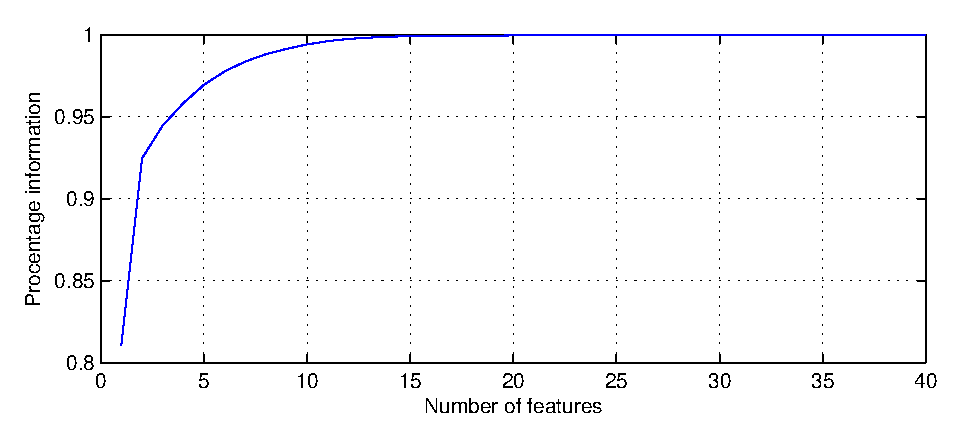
\includegraphics[width=\linewidth]{PCA_dist_var}
\caption{Cumulative distribution of variance (information) in dimensions sorted by highest eigenvalue}
\label{fig:PCA_dist_rap}
\end{figure}

Figure \ref{fig:PCA_dist_rap} shows cumulative distribution of variance in the separate dimensions of the feature space.
In this it is apparent most of the variance is contained within the first 5-10 dimensions. 
$ 94.9 \% $ at 5 dimensions and $ 99.4 \% $ at 10 dimensions.
This does not necessarily imply that most of the information is contained within these, but is a good indicator of this.

In this we see that truncating the feature space to one quarter of the dimensions (10) after PCA, has a very little effect on the overall accuracy of the classification.
This is important, since it can allow the classification algorithms to run with a much lower computational load.
